% !TEX root = QlockToo.tex
% Firmware

\begin{figure}
    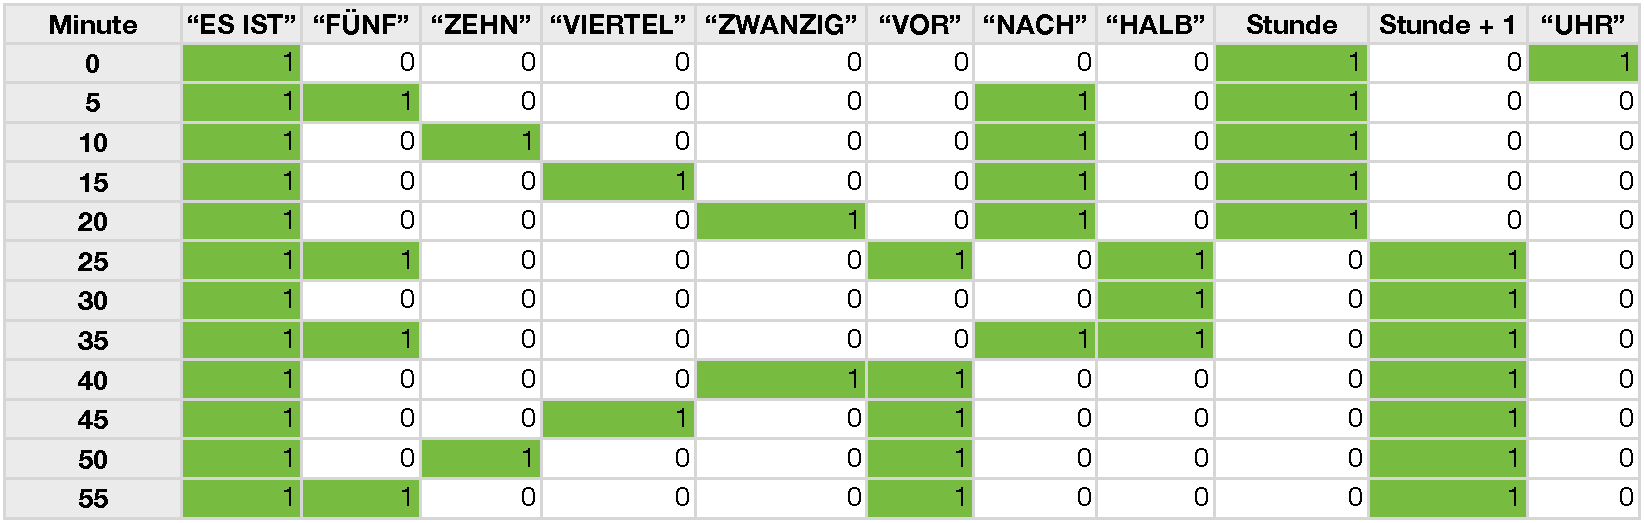
\includegraphics[width=\columnwidth]{Abbildungen/Firmware/Logik}
    \caption{Für die Anzeige der Zeit in Sätzen wird die dargestellte Logiktabelle für die deutsche Sprache in der Firmware hinterlegt. \emph{Stunde} und \emph{Stunde + 1} sind Platzhalter für die aktuelle und die nächste Stunde.}
    \label{fig:Logik}
\end{figure}

\section{Firmware}
\label{sec:Firmware}

\begin{multicols}{2}
Die Firmware der QlockToo ist in C geschrieben und nutzt teilweise Funktionen des Arduino-Cores.
Im Folgenden werden die einzelnen Module der Firmware kurz erläutert.

\textbf{Firmware}

Die Hauptdatei der Firmware enthält den Einstiegspunkt in das Programm und initialisiert alle Module. Hier wird der Haupttimer (1kHz) gestartet, der das Display anzeigt und Steuerungsaufgaben übernimmt.

\textbf{Display}

Im Display-Modul wird die Verbindung mit dem I2C-LED-Treiber hergestellt und die Ports für die Ansteuerung der Leistungstransistoren werden konfiguriert.

In der Display-Update-Routine findet das eigentliche Multiplexing statt. Es wird jeweils die nächste LED-Reihe eingeschaltet und die darzustellenden Spalten über die I2C-Schnittstelle an den LED-Treiber gesendet.
Diese Funktion ist besonders zeitkritisch, da ineffiziente Programmierung hier sofort zu einem flimmernden Bild führt.
Die QlockToo baut das Bild 100 mal pro Sekunde komplett auf (Multiplexing mit 1kHz über zehn Reihen), mit bloßen Auge ist daher kein Flimmern zu erkennen.

\textbf{Timewords}

In diesem Modul ist die in Abbildung~\ref{fig:Logik} dargestellte Logiktabelle implementiert.
Welche LEDs für die gewählten Wörter und Stunden zu beleuchten sind, wird für jedes Wort in Form eines Integers für die Reihe und einer Bitmaske für die Spalten definiert.

\textbf{Api}
Die QlockToo kommuniziert per USB über das UART-Protokoll bei 115200 baud mit der Software.
Zum Parsen der empfangenen Befehle wird auf Seite der Firmware die Library \emph{SerialCommand} eingesetzt.

\textbf{Brightness}

Das Modul Brightness beinhaltet die Steuerung der Helligkeit der QlockToo. Neben dem Automatikmodus, welcher die Helligkeit der  Abhängigkeit von den gemessenen Werten des Helligkeitssensors steuert, besteht die Möglichkeit einer manuellen Steuerung. Dabei stehen sechs Abstufungen zur Verfügung. Aufgrund der Leistungsanpassung sind die Helligkeitsstufen nicht linear.

\textbf{DCF77}

\textbf{Matrix}

\textbf{Settings}

\textbf{Thermo}

\textbf{Time}

\end{multicols}
